% Section: The core: Math
\section{The core: Math}
\label{sec:math}

The Math library (\code{src/core/Math}) holds the numerical objects of \CAP{}: data points and histograms, functions,
fits, extremum searches, random numbers, statistical tests and linear algebra. It replaces the parts of ROOT that
earlier versions of \CAP{} relied on (histograms, \code{TF1}, \code{TGraph}, \code{TProfile}, the fitters and
\code{gRandom}); its sources use only the Base library and the C++ standard library, and include no ROOT header. Its classes are arranged in
eight folders: \code{Basic} (constants, special functions, integration, interpolation, statistics), \code{Data},
\code{Functions}, \code{Fitting}, \code{Search}, \code{Random}, \code{StatisticalTests} and \code{LinearAlgebra}.
Figure~\ref{fig:hierarchy} shows the class hierarchy of the functions and of the data.

\begin{figure}[t]
  \centering
  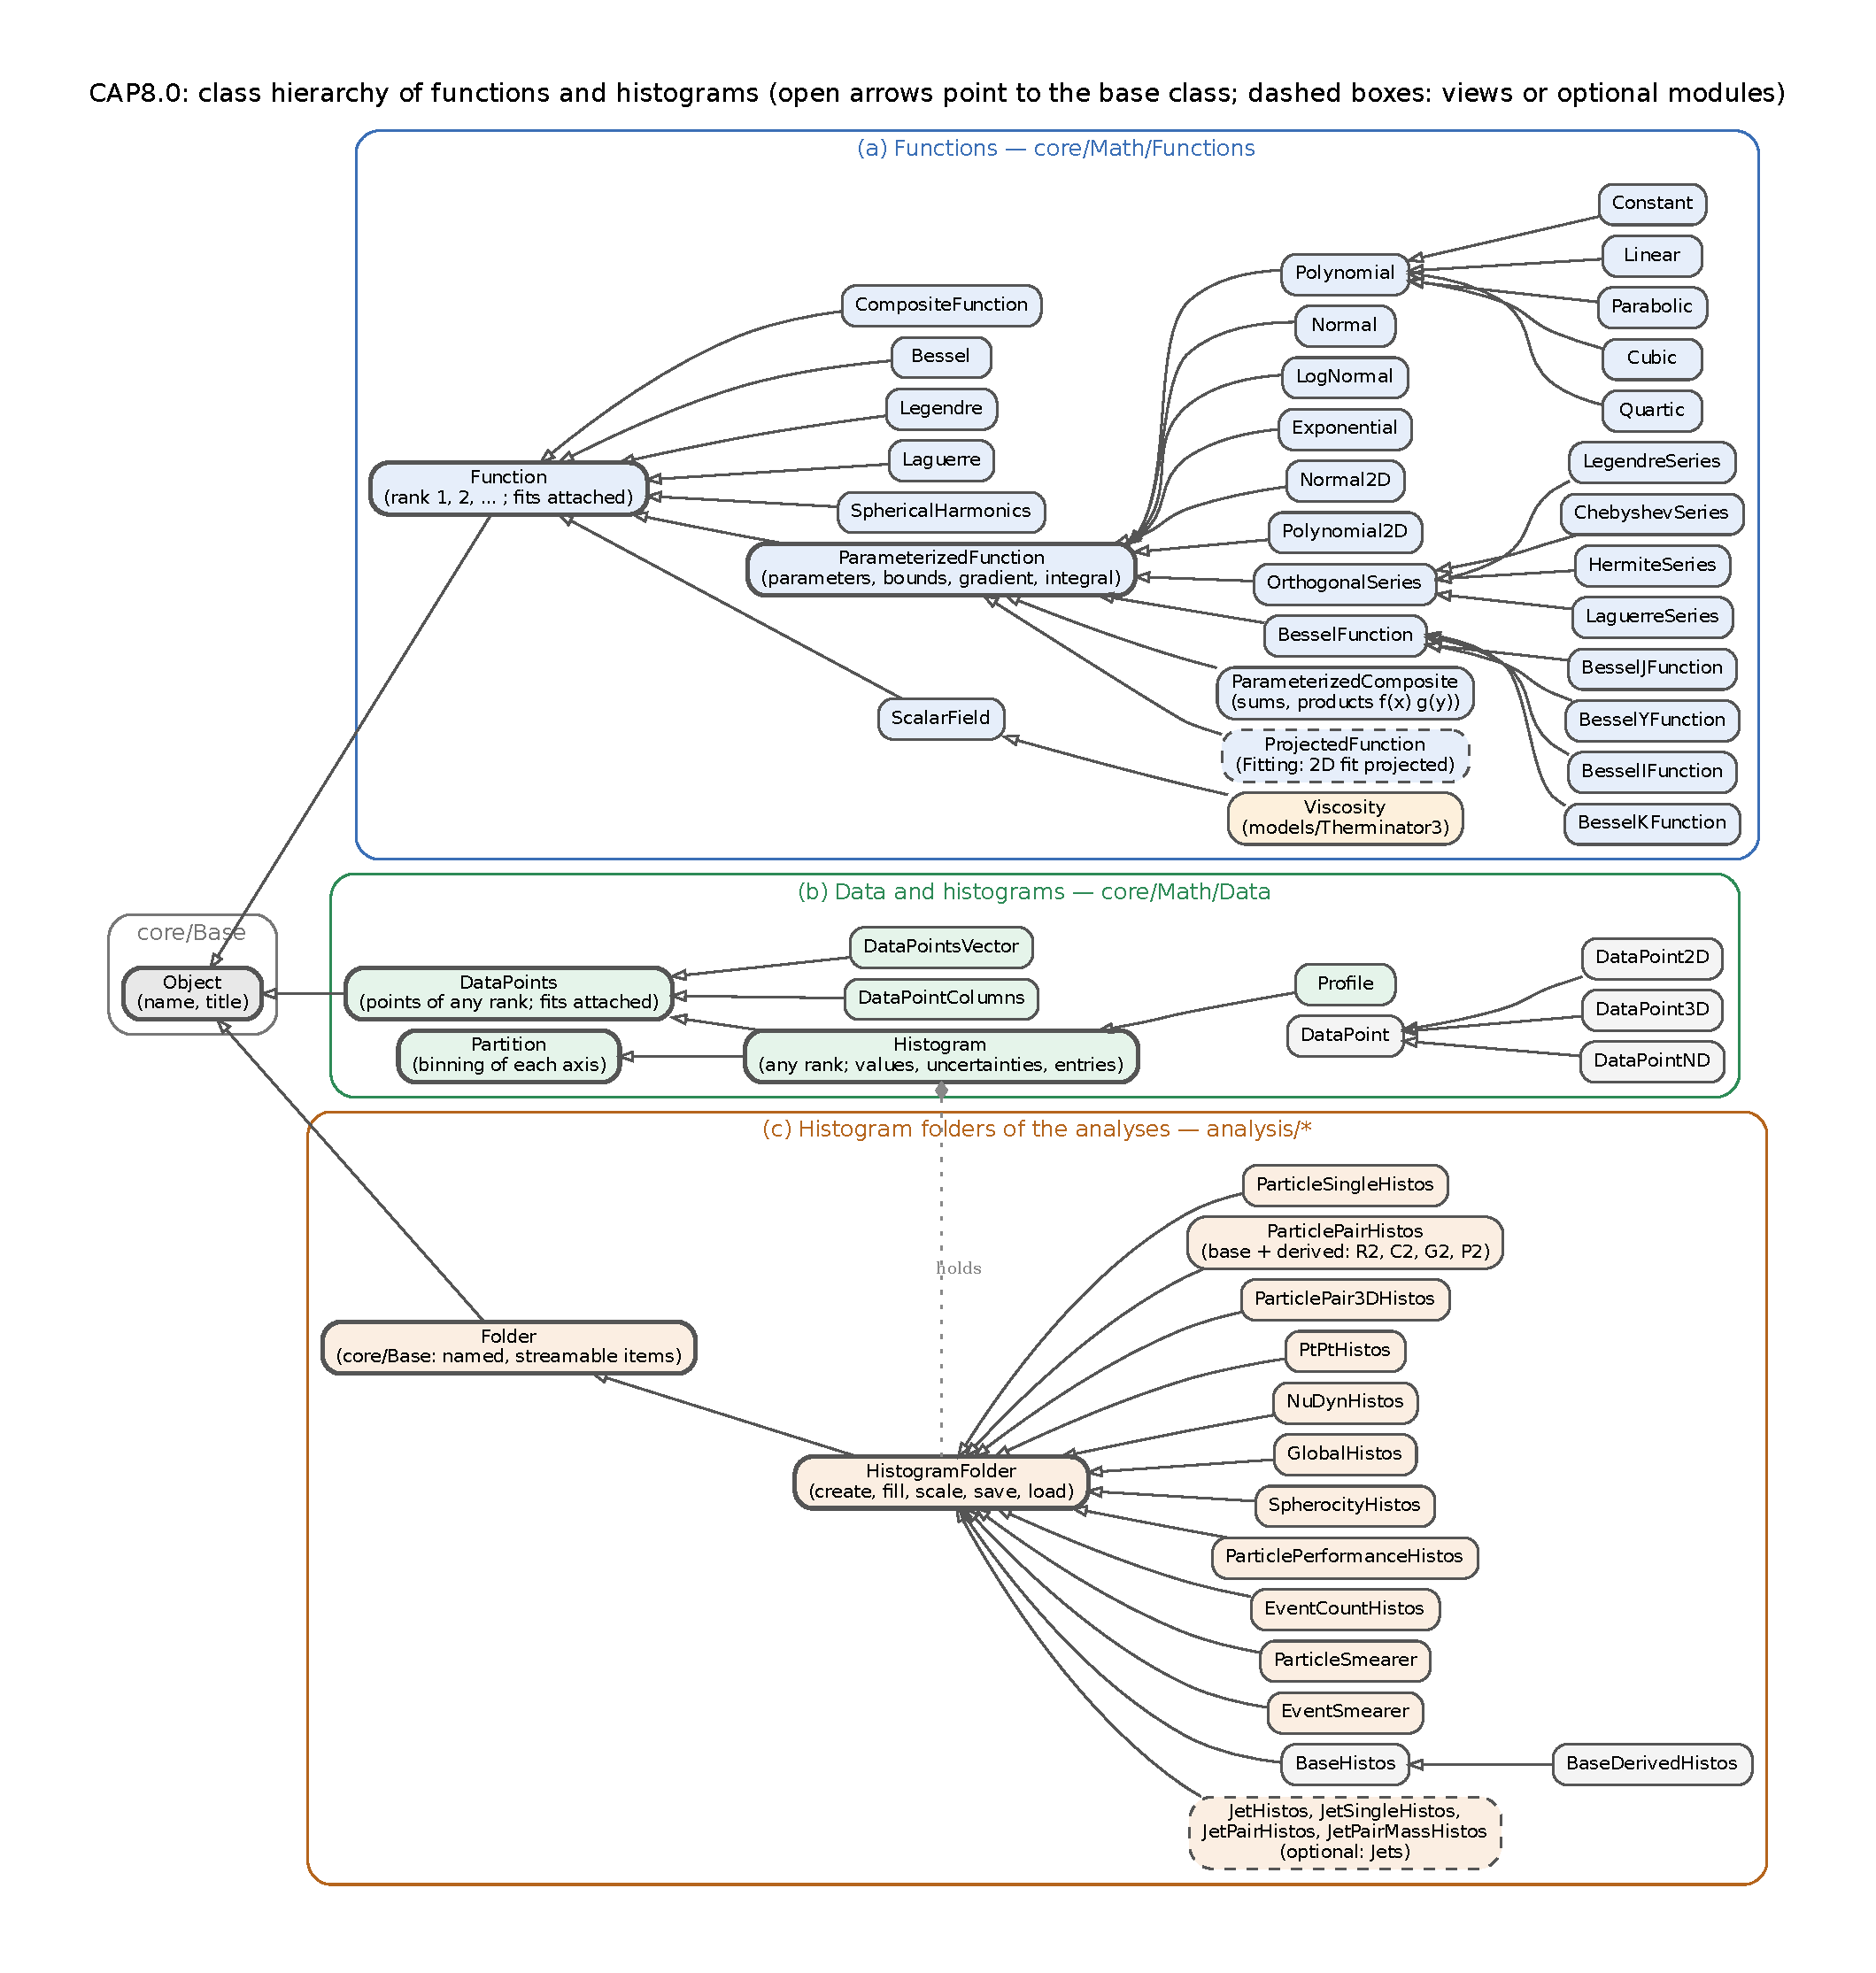
\includegraphics[width=\textwidth]{ClassHierarchy}
  \caption{Class hierarchy of the functions and histograms of \CAP{}~8. Open arrows point to the base class.
  (a)~Functions (\code{core/Math/Functions}); (b)~data points and histograms (\code{core/Math/Data});
  (c)~histogram folders of the analyses (\code{src/analysis}). Dashed boxes are views (\code{ProjectedFunction})
  or optional modules (Jets).}
  \label{fig:hierarchy}
\end{figure}

% ---------------------------------------------------------------------------------------------------------------
\subsection{Data points and histograms}
\label{sec:data}

\paragraph{Data points.}
\code{DataPoints} is the abstract base of every set of measured or computed values. A set has a rank $r$, the number
of its coordinates, and each of its points has coordinates $\mathbf{x}_i = (x_{i,1},\dots,x_{i,r})$ with their
uncertainties, a value $y_i$, a statistical uncertainty $\sigma_i$ and a systematic uncertainty $s_i$. The interface
(\code{coordinatesAt()}, \code{valueAt()}, \code{statErrorAt()}, \code{sysErrorAt()}) is the same for every rank, so
that the fitter, the extremum searches and the graphics work on any set of points without knowing how it is stored.
Two classes store points: \code{DataPointsVector}, a vector of point objects (\code{DataPoint2D},
\code{DataPoint3D}, \code{DataPointND}), and \code{DataPointColumns}, one vector per quantity, which is more compact
for large sets. A set of points also holds the fits made to it (Section~\ref{sec:fitting}).

\paragraph{Partitions.}
The binning of a histogram is a \code{Partition}: a regular partition of a space of any rank, built one axis at a
time. Axis $k$ is divided into $n_k$ bins of equal width over $[a_k, b_k)$. A bin is addressed by its indices
$(i_0, i_1, \dots)$ along the axes, by the coordinates of a point inside it, or by a single global index
\begin{equation}
  g = i_0 + n_0\,\bigl(i_1 + n_1\,(i_2 + \dots)\bigr), \qquad 0 \le g < \prod_k n_k ,
\end{equation}
which is how the bins are stored. Nothing in the classes is specific to one, two or three dimensions: the pair
analyses of Section~\ref{sec:observables} use histograms of rank 2, the three-dimensional pair analysis
histograms of rank 3, and nothing prevents higher ranks.

\paragraph{Histograms.}
\code{Histogram} derives from both \code{DataPoints} and \code{Partition}: a histogram is a set of points, one per bin,
whose coordinates are the centres of the bins, and its binning is a partition. Each bin $g$ stores three numbers:
the number of entries $n_g$ (the number of fills), the average value per entry $a_g$, and the uncertainty $u_g$ of
that average. The bin value and its uncertainty are
\begin{equation}
  y_g = n_g\, a_g, \qquad \sigma_g = n_g\, u_g .
\end{equation}
Filling with a weight $w$ adds $w$ to the value and $w^2$ to its squared uncertainty. Arithmetic (sums,
differences, products, ratios, scaling) acts on the bin values and propagates the statistical uncertainties of
uncorrelated operands; bins where a result is undefined, for instance a ratio with an empty denominator, are left
empty. Values are stored in single or double precision, chosen per histogram, so that the large pair histograms of
an analysis take half the memory when single precision suffices.

The histogram library includes the operations the analyses need on their histograms: integrals over ranges,
projections and reductions (for example from $(\eta_1,\varphi_1,\eta_2,\varphi_2)$ to $(\Delta\eta,\Delta\varphi)$),
symmetrisation, shifts of the $\Delta\varphi$ range, and the computation of the correlation functions of
Section~\ref{sec:observables}: products of single-particle densities, cumulants $C_2$, normalised cumulants $R_2$,
the correlators $\avg{\Delta\pT\Delta\pT}$ and $G_2$, balance functions, and the factorial moments and $\nudyn$ of
multiplicity distributions.

\paragraph{Profiles.}
\code{Profile} derives from \code{Histogram} and holds, in each bin, the weighted mean of a quantity and its
uncertainty. Each bin keeps the sums of the weights $w$, of their squares, of $w v$ and of $w v^2$; the bin value is
the mean and the bin uncertainty the standard error of the mean. Adding two profiles combines these sums, so
merging the profiles of several jobs or sub-samples gives the exact weighted mean.

% ---------------------------------------------------------------------------------------------------------------
\subsection{Functions}
\label{sec:functions}

\paragraph{Functions and parameterised functions.}
\code{Function} is the abstract base of real functions of $r$ real variables, $f(x_1,\dots,x_r)$; $r$ is its rank.
A function is evaluated with one, two or three arguments, or with a vector of arguments, and a call with the wrong
number of arguments throws an exception. \code{ParameterizedFunction} adds a list of parameters,
$f(\mathbf{x};\mathbf{p})$. Each \code{Parameter} has a name, a value, a range and a type that says how it may vary in
a fit: free, fixed, or bounded from below, above or both. A parameterised function provides its gradient
$\nabla_{\mathbf{x}} f$ and its integral over a box; the defaults are numerical (finite differences for the gradient, adaptive Simpson rules for the integrals) and the
functions of the library override them with analytical expressions where these exist. For rank one, the derivative
$f'(x)$ and the mean of $x$ weighted by $f$ over a range are also available.

\paragraph{The library.}
Table~\ref{tab:functions} lists the parameterised functions of \CAP{}. Polynomials of high degree are badly
conditioned in fits; the series of orthogonal polynomials map the range of a fit onto the natural domain of the
polynomials (for example $[-1,1]$ for Legendre and Chebyshev polynomials), where they are nearly orthogonal, and
being linear in their coefficients, their least-squares coefficients are obtained exactly. The library also includes
special functions without parameters (Bessel, Legendre and Laguerre functions, spherical harmonics) and scalar
fields, functions of any rank defined by their values on a regular mesh and interpolated multilinearly, which
Therminator3 uses for its chemical potentials and viscosity (Section~\ref{sec:therminator}).

\begin{widetext}
\begin{table}[t]
  \centering
  \caption{Parameterised functions of \CAP{}~8 (\code{core/Math/Functions}).}
  \label{tab:functions}
  \small
  \begin{tabular}{@{}lll@{}}
    \toprule
    Class & Rank & Form \\
    \midrule
    \code{Polynomial} (\code{Constant} to \code{Quartic}) & 1 & $\sum_{k=0}^{n} c_k x^k$ \\
    \code{Normal} & 1 & $A\, e^{-(x-\mu)^2/2\sigma^2}$ \\
    \code{LogNormal} & 1 & $\dfrac{A}{x\sigma\sqrt{2\pi}}\, e^{-(\ln x-\mu)^2/2\sigma^2}$ \\
    \code{Exponential} & 1 & $a\, e^{b x}$ \\
    \code{LegendreSeries}, \code{ChebyshevSeries} & 1 & $\sum_{k=0}^{N} c_k P_k(t)$, $t\in[-1,1]$ \\
    \code{HermiteSeries} & 1 & $\sum_{k=0}^{N} c_k H_k(t)$ \\
    \code{LaguerreSeries} & 1 & $\sum_{k=0}^{N} c_k L^{\alpha}_k(t)$ \\
    \code{BesselJFunction} (and \code{Y}, \code{I}, \code{K}) & 1 & $A\, Z_n\bigl(k(x-x_0)\bigr)$ \\
    \code{Normal2D} & 2 & $A\exp\!\left[-\dfrac{u^2 - 2\rho u v + v^2}{2(1-\rho^2)}\right]$ \\
    \code{Polynomial2D} & 2 & $\sum_{i+j\le N} c_{ij}\, t^i s^j$ \\
    \code{ParameterizedComposite} & any & $\sum_k f_k(\mathbf{x};\mathbf{p}_k)$, or $f(x)\,g(y)$ \\
    \bottomrule
  \end{tabular}
  \smallskip
  \raggedright\footnotesize In \code{Normal2D}, $u=(x-\mu_x)/\sigma_x$ and $v=(y-\mu_y)/\sigma_y$. In \code{Polynomial2D} and the
  series, $t$ and $s$ are $x$ and $y$ mapped onto the domain of the polynomials.
\end{table}
\end{widetext}

\paragraph{Composite functions.}
A \code{ParameterizedComposite} is a sum of parameterised functions, $f = \sum_k f_k(\mathbf{x};\mathbf{p}_k)$, whose
parameters are those of all its components, named after the label of each component (for example
\code{signal.mean}), or a product of functions of separate variables, such as $f(x)\,g(y)$, a function of two
variables made of two of one. Its derivatives and integrals are those of its components, analytical when theirs
are. A composite can be fitted, copied and stored with its fits like any other function:
\begin{widetext}
\begin{verbatim}[language=C++]
CAP::MATH::ParameterizedComposite model;
model.add("signal",     CAP::MATH::Normal(100.0, 0.0, 1.0));
model.add("background", CAP::MATH::Linear(10.0, 0.0));
CAP::MATH::FunctionRegistry::registerComposite("Gauss+Linear", model);
\end{verbatim}
\end{widetext}
\paragraph{The function registry.}
\code{FunctionRegistry} maps names to classes of parameterised functions and makes new functions by name. It is how
fits are read back from files, which store the name of the class of the fitted function and its parameters, and
how the Fit window of CapGui offers its functions. Programs register their own classes, and composites registered
under a name are kept in a file shared by the programs and CapGui.

% ---------------------------------------------------------------------------------------------------------------
\subsection{Fitting}
\label{sec:fitting}

\paragraph{Statistics.}
A fit finds the parameters $\mathbf{p}$ of a function that minimise a statistic $S(\mathbf{p}) = -2\ln L$, up to a
constant (\code{Likelihood}). Three statistics are provided. For data with Gaussian uncertainties, $S$ is the
$\chi^2$,
\begin{equation}
  \chi^2(\mathbf{p}) = \sum_{i} \frac{\bigl(y_i - f(\mathbf{x}_i;\mathbf{p})\bigr)^2}{V_i},
  \qquad V_i = \sigma_i^2 + s_i^2 + \sum_{k} \left(\frac{\partial f}{\partial x_k}\right)^{\!2} \sigma_{x_k,i}^2 ,
\end{equation}
where the systematic uncertainties $s_i$ and the effective variance from the coordinate uncertainties are included
on request (for rank one, the covariance of $x$ and $y$ is included as well). Points without an uncertainty, such as
the empty bins of a histogram, are left out. For histograms with few entries per bin, the binned Poisson likelihood
ratio of Baker and Cousins~\cite{Baker:1983tu},
\begin{equation}
  S_{\mathrm{P}}(\mathbf{p}) = 2 \sum_{g} \left[ f_g - n_g + n_g \ln\frac{n_g}{f_g} \right],
\end{equation}
is unbiased where the $\chi^2$ is not, includes the empty bins, and is asymptotically $\chi^2$-distributed. For
individual events, the unbinned likelihood takes the function as the density of the events over a range $\Omega$,
\begin{equation}
  S_{\mathrm{U}} = -2\sum_{i} \ln\frac{f(\mathbf{x}_i;\mathbf{p})}{N(\mathbf{p})}, \qquad
  S_{\mathrm{E}} = 2N(\mathbf{p}) - 2\sum_{i} \ln f(\mathbf{x}_i;\mathbf{p}), \qquad
  N(\mathbf{p}) = \int_{\Omega} f(\mathbf{x};\mathbf{p})\, d\mathbf{x},
\end{equation}
without and with extension ($S_{\mathrm{E}}$, where $N$ is the expected number of events and the amplitude is
fitted). For histograms whose bins are wide compared to the structures fitted, the function can be compared to its
average over each bin, computed with a three-point Gauss--Legendre rule along each axis, rather than to its value at
the centre of the bin.

\paragraph{Ranges and regions.}
A fit uses the points in a selection (\code{FitSelection}): a box, $a_k \le x_k \le b_k$ for each variable, regions
included, and regions excluded. A region is a set of intervals along some of the variables, the others not being
restricted, so that it is a band, a slab or a box. A point, or the centre of a bin, is used if it is in the box, in at
least one included region (if there is any), and in no excluded region. Excluding a region leaves out a peak or a
dead area; including two regions fits two sidebands. For an unbinned fit, the normalisation $N(\mathbf{p})$ is the
integral over the selection: the box is split into cells at the ends of the intervals of the regions, each cell is
either wholly in or wholly out of the selection, and $N$ is the sum of the integrals over the cells that are in.

\paragraph{Minimisation.}
The default method is Levenberg--Marquardt. For a statistic made of residuals $r_i$ ($\chi^2$ and Poisson
likelihood, whose residuals are the pulls and the signed deviance residuals), each step solves
\begin{equation}
  \bigl(J^{\mathsf{T}}J + \lambda\,\mathrm{diag}(J^{\mathsf{T}}J)\bigr)\,\delta\mathbf{p} = -J^{\mathsf{T}}\mathbf{r},
\end{equation}
where $J_{ia} = \partial r_i/\partial p_a$ is computed by central differences (one-sided at a bound), and the damping
$\lambda$ grows tenfold until $S$ decreases and shrinks tenfold after each successful step. For the unbinned
likelihood, which is not a sum of squares, the same scheme is applied to the numerical gradient and curvature of
$S$. Fixed parameters keep their values, and bounded parameters stay within their bounds. When the starting values
are poor or $S$ has several minima, a global search (Section~\ref{sec:mathother}), such as differential evolution
over the bounds of the free parameters, runs first and Levenberg--Marquardt refines its result. Starting values can
also be estimated from the data in the selection for the common functions: moments for Gaussian peaks, a straight
line in $\ln y$ for an exponential, exact least squares for polynomials and series.

\paragraph{Uncertainties.}
The covariance of the free parameters at the minimum is $C = (J^{\mathsf{T}}J)^{-1}$ for a statistic made of residuals,
and $C = 2H^{-1}$ otherwise, $H$ being the curvature of $S$. It can be scaled by $\chi^2/\nu$ when the uncertainties
of the data are known only up to a factor. The result of a fit (\code{FitResult}) holds the values, uncertainties,
covariance and correlation matrices of the parameters, the statistic, the number of degrees of freedom $\nu$ and,
for the binned statistics, the $p$-value of the $\chi^2$ distribution, together with flags for convergence and for
parameters at a bound.

\paragraph{Bayesian fits.}
\code{BayesianFitter} samples the posterior distribution of the parameters,
\begin{equation}
  p(\mathbf{p}\,|\,\text{data}) \propto L(\mathbf{p})\,\prod_a \pi_a(p_a),
\end{equation}
with priors $\pi_a$ that are flat, uniform, Gaussian (for instance an earlier
measurement), log-uniform for a scale of unknown magnitude, or any log density. The sampler is an adaptive
Metropolis--Hastings algorithm: several chains (four by default) start near the starting values; during the burn-in
the size of the proposals adapts to a target acceptance of 0.25, and halfway through it their covariance becomes that
of the samples drawn so far, so that correlated parameters are sampled efficiently. The result gives, for each
parameter, its mean, spread, quantiles, credible intervals and mode, the covariance of the samples, and the
diagnostics of the chains: acceptance, effective sample size and $\hat{R}$.

\paragraph{Fits attached to the objects fitted.}
A fit is kept with the object it was made to, data points, a histogram or a function, as a \code{FitRecord}: a copy of
the fitted function at the best parameters, the result, a label, the box covered by the points used and the regions
of the selection. The records are written to and read from CAP files with the object (Section~\ref{sec:binary}),
the function being recreated through the registry, so that a fit made in a program is drawn and inspected in
CapGui, and the reverse. The residuals of a fit, $y_i - f(\mathbf{x}_i)$ or the pulls, are computed for the points
used, and the fits of rank two of a histogram can be projected onto either axis with the histogram:
\begin{verbatim}[language=C++]
CAP::MATH::Normal model(100.0, 0.0, 1.0);            // starting values
CAP::MATH::Fitter fitter(model, histogram);          // chi square by default
fitter.exclude(0, 4.5, 5.5);                         // leave a region out
CAP::MATH::FitResult r = fitter.fit();
histogram.addFit(fitter.record("gaussian"));         // saved with the histogram
\end{verbatim}

% ---------------------------------------------------------------------------------------------------------------
\subsection{Searches, random numbers, statistical tests and linear algebra}
\label{sec:mathother}

\paragraph{Extremum searches.}
\code{ExtremumSearch} finds the minimum or maximum of a function or of a set of data points over a domain with
bounds and excluded regions. Local methods (gradient, hill climbing, greedy) start from a point; global methods (scan,
simulated annealing, genetic algorithm, differential evolution, divide and conquer, explore--exploit) need a bounded
domain. A second method can refine the result of the first, a method can be run from several starting points, and
for histograms the extremum is placed between bins by a parabolic fit. The fitter uses these engines for its global
searches.

\paragraph{Random numbers.}
\code{RandomGenerator} draws the common distributions (Gaussian, exponential, Poisson, binomial, gamma, beta,
$\chi^2$, polynomial densities) from the uniform numbers of any engine; the engine provided is the Mersenne Twister
MT19937, whose state can be saved and restored to continue a sequence. New distributions derive from
\code{RandomDistribution} and work with every engine.

\paragraph{Statistical tests.}
Binomial, Poisson, Gaussian, Student $t$ and $\chi^2$ tests, the compatibility of two histograms, and the
Kolmogorov--Smirnov test are provided, with one- or two-sided alternatives, together with the cumulative
distributions they need. Upper tails are computed directly, so that small $p$-values keep their precision.

\paragraph{Linear algebra and kinematics.}
\code{Matrix} provides the dense matrices of the fits (products, inverses, determinants), and \code{Vector2D},
\code{Vector3D}, \code{VectorND} and \code{VectorLorentz} the vectors and four-vectors of particle kinematics, with
the $(+,-,-,-)$ metric and $c=1$.

\todo{decide whether to add a short paragraph on Basic (integration, interpolation, robust moments) and a figure
of a fit with an excluded region drawn by CapGui.}
